\setcounter{tocdepth}{4}
\setcounter{secnumdepth}{4}

\subsubsection{List of requirements}

\arrayrulecolor{tableBorderColor}
\setlength\arrayrulewidth{1pt}
\rowcolors{2}{white}{tableHighlightColor}
\setlength\LTleft{0pt}

\begin{longtable}{ !\Vline c !\Vline p{0.9\linewidth} !\Vline}
    \hline
    \textbf{R1} & Users certified with an authentication\\
    \textbf{R2} & Managers certified with an authentication\\
    \textbf{R3} & Managers should register to the application with extra mandatory fields\\
    \textbf{R4} & Only managers can create shop\\
    \textbf{R5} & Only managers can update their shop\\
    \textbf{R6} & Managers can activate advance function 1 (allow users booking) on their shop\\
    \textbf{R7} & Managers can activate advance function 2 (send suggestions) on their shop\\
    \textbf{R8} & Users must accept the GPS location for the application\\
    \textbf{R9} & Users could see the list of shops are around them\\
    \textbf{R10} & Users could go to current line-up queue for specific shop \\
    \textbf{R11} & Users could see their ticket (QR code) and estimated waiting time \\
    \textbf{R12} & Users could choose book a time to visit specific shop \\
    \textbf{R13} & Users could choose for which categories they go shopping when they book a visit \\
    \textbf{R14} & The system must generate suitable QR code\\
    \textbf{R15} & The system must estimate the waiting time for each user\\
    \textbf{R16} & The system must make current line-up queue based on users booking\\
    \textbf{R17} & The system sends a notification to user to approach shop based on current location of user and location of shop\\
    \textbf{R18} & The system sends a notification to user to go to the shop when it's him/her turn\\
    \textbf{R19} & After user ticket scanned for entrance, system change status of ticket to invalidate for entrance\\
    \textbf{R20} & The clerk must scan the user ticket\\
    \textbf{R21} & The clerk could add a person to current line-up queue\\
    \textbf{R22} & The clerk could print ticket\\
    \textbf{R23} & After the user checked out, the system analyze shopping list and duration time and add it to the user's visit history \\
    \textbf{R24} & The system could estimate the category of shopping and duration of shopping for specific user \\
    \textbf{R25} & The system estimate the time based on user characteristic\\
    \textbf{R26} & Users can ask a clerk to give them a ticket\\
    \textbf{R27} & If specific time past from user turn to enter his/her ticket will be invalidate for entrance\\
    \textbf{R28} & If managers update a shop the estimated time and book visits will be recalculate\\
    \textbf{R29} & Manager choose the capacity of shop\\
    \textbf{R30} & Manager choose the category of each section in the shop and their capacity\\
    \textbf{R31} & Manager choose working hour of the shop\\
    \hline
\end{longtable}

\subsubsection{Mapping}
\arrayrulecolor{tableBorderColor}
\setlength\arrayrulewidth{1pt}
\rowcolors{2}{white}{tableHighlightColor}
\setlength\LTleft{0pt}
\begin{longtable}{ !\Vline c !\Vline p{0.45\linewidth} !\Vline p{0.45\linewidth} !\Vline}
    \hline
    \multicolumn{1}{|c|}{\textbf{Goal}} & \multicolumn{1}{c|}{\textbf{Domain assumption}} & \multicolumn{1}{c|}{\textbf{Requirements}}\\
    G1 & D1,D2,D4,D6,D10,D11 & R1,R9,R10,R11,R14,R16\\
    G1 & D1,D2,D6,D7,D8,D9,D10,D12 & R1,R9,R11,R12,R13,R14,R16,R21,R22\\
    
    \hline
\end{longtable}

\subsubsection{Use cases}
\paragraph{Use case Description} \hfill
\begin{itemize}

\item \textbf{Register}
\arrayrulecolor{tableBorderColor}
\setlength\arrayrulewidth{1pt}
\rowcolors{2}{white}{tableHighlightColor}
\setlength\LTleft{0pt}
\begin{longtable}{ !\Vline c !\Vline p{0.9\linewidth} !\Vline}
    \hline
    \textbf{Name} & \textbf{Register}\\
    \textbf{ID} & UC1\\
    \textbf{Actors} & Super User\\
    \textbf{Entry Condition} & Super User has internet connection on his/her device\\
    \textbf{Event flow} & 
    \begin{enumerate}
        \item Super user see the landing page
        \item Super user click on the "sign up" button
        \item Super user fill all the mandatory fields
        \item Super user choose his type between manager or user
        \item Super user fill extra fields based on his type
        \item Super user click on "Register" button
        \item The system validate the filled data
        \item The system confirm the registration
        \item The system save the super user on database
    \end{enumerate}\\
    \textbf{Exit Condition} & Super user is successfully registered in the system\\
    \textbf{Exceptions} & 
    If the below conditions happened the application return a suitable error in message and return to register page.
    \begin{itemize}
        \item Super user is already existed in the system
        \item Super user doesn't fill all mandatory fields
        \item Super user sends invalid data
    \end{itemize}
    
    \\
    \hline
\end{longtable}

\item \textbf{Login}
\arrayrulecolor{tableBorderColor}
\setlength\arrayrulewidth{1pt}
\rowcolors{2}{white}{tableHighlightColor}
\setlength\LTleft{0pt}
\begin{longtable}{ !\Vline c !\Vline p{0.9\linewidth} !\Vline}
    \hline
    \textbf{Name} & \textbf{Login}\\
    \textbf{ID} & UC2\\
    \textbf{Actors} & Super User\\
    \textbf{Entry Condition} & Super User has internet connection and it already registered to the application\\
    \textbf{Event flow} & 
    \begin{enumerate}
        \item Super user see the landing page
        \item Super user click on the "sign in" button
        \item Super user fill username and password fields
        \item Super user click on "Login" button
        \item The system check the credential
        \item The system confirm the registration
        \item The system return the home page of user
    \end{enumerate}\\
    \textbf{Exit Condition} & Super user has access to the service of CLup\\
    \textbf{Exceptions} & 
    If the below conditions happened the application return a suitable error in message and return to login page.
    \begin{itemize}
        \item Super user is not exist in the system
        \item Super user doesn't fill all mandatory fields
        \item Super user password is invalid
    \end{itemize}
    
    \\
    \hline
\end{longtable}

\item \textbf{Create shop}
\arrayrulecolor{tableBorderColor}
\setlength\arrayrulewidth{1pt}
\rowcolors{2}{white}{tableHighlightColor}
\setlength\LTleft{0pt}
\begin{longtable}{ !\Vline c !\Vline p{0.9\linewidth} !\Vline}
    \hline
    \textbf{Name} & \textbf{Create Shop}\\
    \textbf{ID} & UC3\\
    \textbf{Actors} & Manager\\
    \textbf{Entry Condition} & Manager has internet connection\\
    \textbf{Event flow} & 
    \begin{enumerate}
        \item Manager see the home page
        \item Manager click on the "add a shop" button
        \item Manager set shop title
        \item Manager set location of the shop
        \item Manager set start and end hour of the shop
        \item Manager set capacity of the shop
        \item manager click on "new category"
        \item manager set capacity and title of category
        \item click on "end" button or return to 7.
        \item manager choose AF1 or AF2 enable by checkbox.
        \item manager click on "Submit" button.
        \item The system shows all the detail of shop.
        \item manager click on "Accept" button.
        \item The system add shop to data base.
    \end{enumerate}\\
    \textbf{Exit Condition} & Shop successfully created\\
    \textbf{Exceptions} & If the data of shop is not valid the sytem will return error\\
    \hline
\end{longtable}

\item \textbf{Update shop}
\arrayrulecolor{tableBorderColor}
\setlength\arrayrulewidth{1pt}
\rowcolors{2}{white}{tableHighlightColor}
\setlength\LTleft{0pt}
\begin{longtable}{ !\Vline c !\Vline p{0.9\linewidth} !\Vline}
    \hline
    \textbf{Name} & \textbf{Create Shop}\\
    \textbf{ID} & UC4\\
    \textbf{Actors} & Manager\\
    \textbf{Entry Condition} & Manager has internet connection and the shop is exists\\
    \textbf{Event flow} & 
    \begin{enumerate}
        \item Manager see the home page
        \item Manager click on the "edit" button in specific shop
        \item Manager change fields it like
        \item manager click on "Submit" button.
        \item The system shows all the detail of shop.
        \item manager click on "Accept" button.
        \item The system update the shop in data base.
        \item The system update recalculate the estimated time by new values.
    \end{enumerate}\\
    \textbf{Exit Condition} & Shop successfully updated\\
    \textbf{Exceptions} & 
        If the below conditions happened the application return a suitable error.
    \begin{itemize}
        \item Shop is not existed in the system.
        \item Manager doesn't have access to change that shop.
        \item Fields values are invalid.
    \end{itemize}\\
    \hline
\end{longtable}

\item \textbf{See list of shops}
\arrayrulecolor{tableBorderColor}
\setlength\arrayrulewidth{1pt}
\rowcolors{2}{white}{tableHighlightColor}
\setlength\LTleft{0pt}
\begin{longtable}{ !\Vline c !\Vline p{0.9\linewidth} !\Vline}
    \hline
    \textbf{Name} & \textbf{See list of shops}\\
    \textbf{ID} & UC5\\
    \textbf{Actors} & User\\
    \textbf{Entry Condition} & User has internet connection and must accept GPS permission\\
    \textbf{Event flow} & 
    \begin{enumerate}
        \item User get latitude and longitude from GPS
        \item User send a request to get list of shops
        \item The system extract latitude and longitude from user request
        \item The system get shop list from database
        \item The system order shops based on latitude and longitude and characteristic of user.
        \item The system shows the list of shops to user.
    \end{enumerate}\\
    \textbf{Exit Condition} & User see list of shops\\
    \textbf{Exceptions} & None\\
    \hline
\end{longtable}


\item \textbf{Generate ticket}
\arrayrulecolor{tableBorderColor}
\setlength\arrayrulewidth{1pt}
\rowcolors{2}{white}{tableHighlightColor}
\setlength\LTleft{0pt}
\begin{longtable}{ !\Vline c !\Vline p{0.9\linewidth} !\Vline}
    \hline
    \textbf{Name} & \textbf{Generate ticket}\\
    \textbf{ID} & UC6\\
    \textbf{Actors} & User, Clerk\\
    \textbf{Entry Condition} & user or clerk wants to add to a line-up queue\\
    \textbf{Event flow} & 
    \begin{enumerate}
        \item The system extract the user turn.
        \item The system extract the user id.
        \item The system extract the shop id.
        \item The system extract the line-up queue id.
        \item The system generate a QR code based on those information.
        \item The system saves generated QR code to database.
        \item The system shows the generated QR code to user.
    \end{enumerate}\\
    \textbf{Exit Condition} & QR code generated successfully \\
    \textbf{Exceptions} & None\\
    \hline
\end{longtable}

\item \textbf{Estimate waiting time}
\arrayrulecolor{tableBorderColor}
\setlength\arrayrulewidth{1pt}
\rowcolors{2}{white}{tableHighlightColor}
\setlength\LTleft{0pt}
\begin{longtable}{ !\Vline c !\Vline p{0.9\linewidth} !\Vline}
    \hline
    \textbf{Name} & \textbf{Estimate waiting time}\\
    \textbf{ID} & UC7\\
    \textbf{Actors} & User, Clerk\\
    \textbf{Entry Condition} & user or clerk wants to add to a line-up queue\\
    \textbf{Event flow} & 
    \begin{enumerate}
        \item The system extract the users from line-up queue.
        \item The system extract the shop.
        \item The system extract the new user wants to add in line up.
        \item The system get history of users shopping from database.
        \item The system extract new user wants shop from which categories.
        \item based on previous behavior of user and categories system estimate shopping duration of user.
        \item based on previous users in queue, system estimate waiting time for user.
    \end{enumerate}\\
    \textbf{Exit Condition} & The system estimate the user waiting time \\
    \textbf{Exceptions} & Check the shops, users and line-up queue are really exists. if they are not exist send a proper message.\\
    \hline
\end{longtable}

\item \textbf{Add to Line-up Queue}
\arrayrulecolor{tableBorderColor}
\setlength\arrayrulewidth{1pt}
\rowcolors{2}{white}{tableHighlightColor}
\setlength\LTleft{0pt}
\begin{longtable}{ !\Vline c !\Vline p{0.9\linewidth} !\Vline}
    \hline
    \textbf{Name} & \textbf{Add to Line-up Queue}\\
    \textbf{ID} & UC8\\
    \textbf{Actors} & User, Clerk\\
    \textbf{Entry Condition} & user choose specific shop to go to one of it lines up queue or user book a visit, clerk wants to add person do not use application to a line-up queue\\
    \textbf{Event flow} & 
    \begin{enumerate}
        \item User choose a shop to add line up or book a visit for that shop or clerk click on add to line-up.
        \item The system find that line-up queue
        \item The system get the generate number of user in queue.
        \item The system pass user, shop and queue to [UC6].
        \item The system get the QR code of ticket.
        \item The system pass user, shop and queue to [UC7].
        \item The system get the estimation waiting time for user.
        \item The system get current location of user.
        \item The system get calculate traveling time estimation for user.
        \item The system set interval to send notification for approach a user.
        \item The system add user to correct line-up queue.
        \item The system send ticket and estimated time to user.
    \end{enumerate}\\
    \textbf{Exit Condition} & add user to line-up queue \\
    \textbf{Exceptions} & None\\
    \hline
\end{longtable}

\item \textbf{Book a visit}
\arrayrulecolor{tableBorderColor}
\setlength\arrayrulewidth{1pt}
\rowcolors{2}{white}{tableHighlightColor}
\setlength\LTleft{0pt}
\begin{longtable}{ !\Vline c !\Vline p{0.9\linewidth} !\Vline}
    \hline
    \textbf{Name} & \textbf{Book a visit}\\
    \textbf{ID} & UC9\\
    \textbf{Actors} & User\\
    \textbf{Entry Condition} & The shop AF1 is activate and user choose book\\
    \textbf{Event flow} & 
    \begin{enumerate}
        \item User choose a shop.
        \item User click on "book a visit" button.
        \item The user choose date and time.
        \item The system returns items' category of that shop.
        \item User add category of items wants to buy.
        \item Based on date user choose system finds a suitable queue.
        \item Pass the parameters to [UC8] and get the result.
        \item Get the ticket and show it.
    \end{enumerate}\\
    \textbf{Exit Condition} & user successfully book a visit \\
    \textbf{Exceptions} & If user the queue capacity is full\\
    \hline
\end{longtable}

\item \textbf{See ticket}
\arrayrulecolor{tableBorderColor}
\setlength\arrayrulewidth{1pt}
\rowcolors{2}{white}{tableHighlightColor}
\setlength\LTleft{0pt}
\begin{longtable}{ !\Vline c !\Vline p{0.9\linewidth} !\Vline}
    \hline
    \textbf{Name} & \textbf{See ticket}\\
    \textbf{ID} & UC10\\
    \textbf{Actors} & User\\
    \textbf{Entry Condition} & The user has a ticket for that shop\\
    \textbf{Event flow} & 
    \begin{enumerate}
        \item User choose a shop.
        \item User click on "ticket" button.
        \item The system find the ticket.
        \item The system calculate remaining time.
        \item The system return the QR code and estimation time.
    \end{enumerate}\\
    \textbf{Exit Condition} & user get the ticket \\
    \textbf{Exceptions} & If user is doesn't have the ticket for that shop system return a message\\
    \hline
\end{longtable}

\item \textbf{Notify user for approach}
\arrayrulecolor{tableBorderColor}
\setlength\arrayrulewidth{1pt}
\rowcolors{2}{white}{tableHighlightColor}
\setlength\LTleft{0pt}
\begin{longtable}{ !\Vline c !\Vline p{0.9\linewidth} !\Vline}
    \hline
    \textbf{Name} & \textbf{Notify user for approach}\\
    \textbf{ID} & UC11\\
    \textbf{Actors} & Time\\
    \textbf{Entry Condition} & Timer that [UC8] set, finished\\
    \textbf{Event flow} & 
    \begin{enumerate}
        \item The system sends a request to notification system.
        \item The notification system send a notification to user.
    \end{enumerate}\\
    \textbf{Exit Condition} & user get notification \\
    \textbf{Exceptions} & none\\
    \hline
\end{longtable}

\item \textbf{Print ticket}
\arrayrulecolor{tableBorderColor}
\setlength\arrayrulewidth{1pt}
\rowcolors{2}{white}{tableHighlightColor}
\setlength\LTleft{0pt}
\begin{longtable}{ !\Vline c !\Vline p{0.9\linewidth} !\Vline}
    \hline
    \textbf{Name} & \textbf{Print ticket}\\
    \textbf{ID} & UC13\\
    \textbf{Actors} & Clerk\\
    \textbf{Entry Condition} & A person doesn't use mobile ask clerk for a ticket\\
    \textbf{Event flow} & 
    \begin{enumerate}
        \item The clerk click "ticket" on ticket machine.
        \item The system add an anonymous user to queue by [UC9].
        \item The system show ticket.
        \item The clerk click on "print" button.
        \item The printer print the ticket.
    \end{enumerate}\\
    \textbf{Exit Condition} & anonymous user got to queue and ticket printed\\
    \textbf{Exceptions} & none\\
    \hline
\end{longtable}

\item \textbf{Scan QR code for entrance}
\arrayrulecolor{tableBorderColor}
\setlength\arrayrulewidth{1pt}
\rowcolors{2}{white}{tableHighlightColor}
\setlength\LTleft{0pt}
\begin{longtable}{ !\Vline c !\Vline p{0.9\linewidth} !\Vline}
    \hline
    \textbf{Name} & \textbf{Scan QR code for entrance}\\
    \textbf{ID} & UC14\\
    \textbf{Actors} & Clerk\\
    \textbf{Entry Condition} & A person want to enter the shop\\
    \textbf{Event flow} & 
    \begin{enumerate}
        \item The person show his/her ticket on mobile or printed ticket.
        \item The clerk scan QR code.
        \item The system check can the user enter.
        \item The system remove user from line-up queue.
        \item The system change ticket status invalid for entrance.
        \item The system set start time for user.
    \end{enumerate}\\
    \textbf{Exit Condition} & user can enter the shop\\
    \textbf{Exceptions} & If it isn't user turn red flash light blink on scanner\\
    \hline
\end{longtable}

\item \textbf{checkout}
\arrayrulecolor{tableBorderColor}
\setlength\arrayrulewidth{1pt}
\rowcolors{2}{white}{tableHighlightColor}
\setlength\LTleft{0pt}
\begin{longtable}{ !\Vline c !\Vline p{0.9\linewidth} !\Vline}
    \hline
    \textbf{Name} & \textbf{checkout}\\
    \textbf{ID} & UC15\\
    \textbf{Actors} & Clerk\\
    \textbf{Entry Condition} & A person want to checkout the shop\\
    \textbf{Event flow} & 
    \begin{enumerate}
        \item The person show his/her ticket on mobile or printed ticket.
        \item The clerk scan QR code.
        \item The system find the user.
        \item The clerk scan bar code of items with his/her scanner.
        \item The system find category of items and add to user history.
        \item The system set end time for user and calculate the duration.
        \item The system add user history to database.
        \item The system call the next person turn.
        \item The system set a 1 minute timer to notify next person.
    \end{enumerate}\\
    \textbf{Exit Condition} & user checkout and exit the shop\\
    \textbf{Exceptions} & If user lost his ticket act him as an anonymous user.\\
    \hline
\end{longtable}

\item \textbf{checkout}
\arrayrulecolor{tableBorderColor}
\setlength\arrayrulewidth{1pt}
\rowcolors{2}{white}{tableHighlightColor}
\setlength\LTleft{0pt}
\begin{longtable}{ !\Vline c !\Vline p{0.9\linewidth} !\Vline}
    \hline
    \textbf{Name} & \textbf{checkout}\\
    \textbf{ID} & UC16\\
    \textbf{Actors} & Time\\
    \textbf{Entry Condition} & Timer that [UC15] set finished.\\
    \textbf{Event flow} & 
    \begin{enumerate}
        \item The system change ticket of user to valid.
        \item The system sends a request to notification system.
        \item The notification system send a notification to user.
    \end{enumerate}\\
    \textbf{Exit Condition} & user get notification\\
    \textbf{Exceptions} & None\\
    \hline
\end{longtable}

\end{itemize}
\clearpage

\paragraph{Use case Diagram} \mbox{} \\
\begin{figure}[H]
  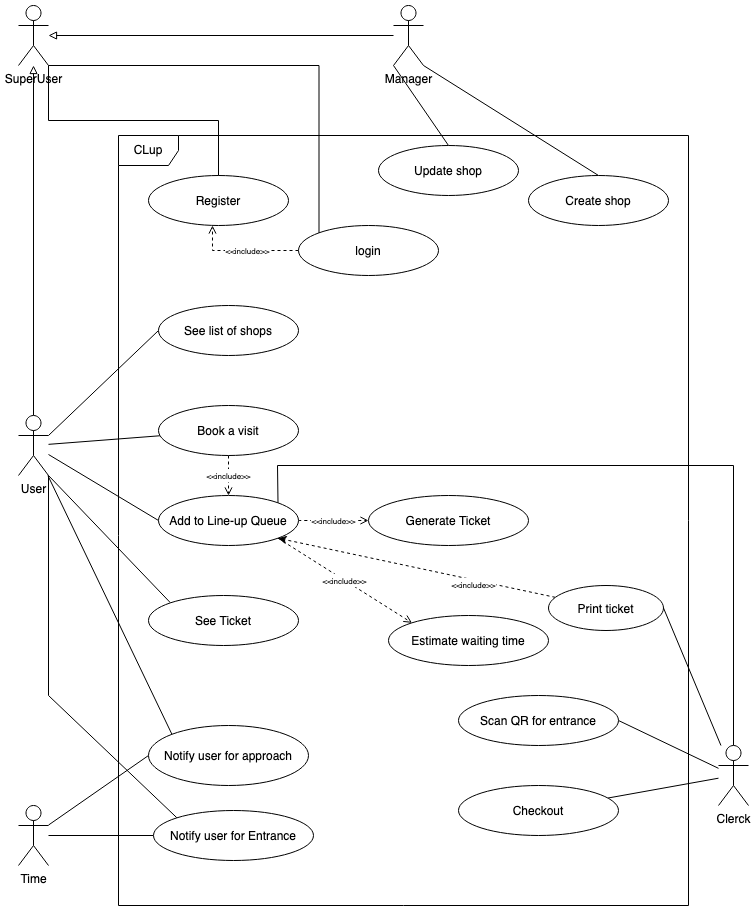
\includegraphics[width=\textwidth,height=\textheight,keepaspectratio]{images/Usecase.png}
  \caption{Use case diagram}
  \label{fig:usecase}
\end{figure}
\clearpage

\subsubsection{Sequence Diagrams}

\begin{figure}[H]
  \centering
  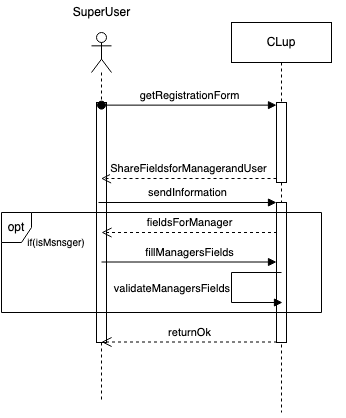
\includegraphics[width=0.5\textwidth,keepaspectratio]{images/Register_sd.png}
  \caption{Sequence diagram for register}
\end{figure}

\begin{figure}[H]
  \centering
  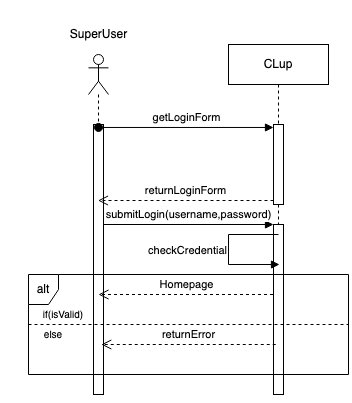
\includegraphics[width=0.5\textwidth,keepaspectratio]{images/login_sd.png}
  \caption{Sequence diagram for login}
\end{figure}

\begin{figure}[H]
  \centering
  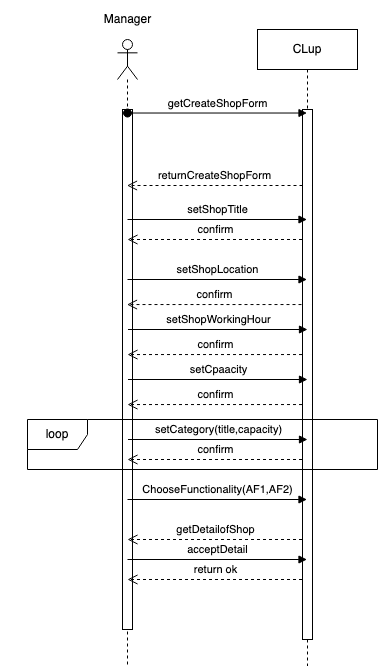
\includegraphics[width=0.8\textwidth,keepaspectratio]{images/CreateShop_sd.png}
  \caption{Sequence diagram for create a shop}
\end{figure}

\begin{figure}[H]
  \centering
  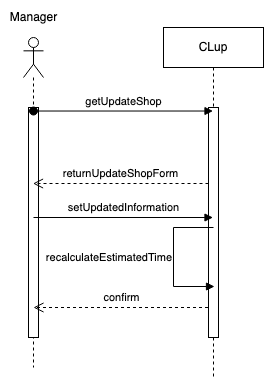
\includegraphics[width=0.5\textwidth,keepaspectratio]{images/UpdateShop_sd.png}
  \caption{Sequence diagram for update shop}
\end{figure}

\begin{figure}[H]
  \centering
  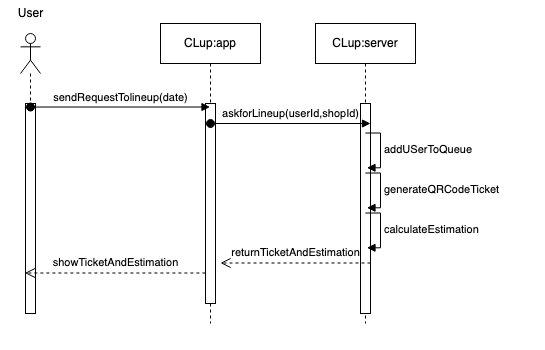
\includegraphics[width=0.8\textwidth,keepaspectratio]{images/AddToLineUp_sd.png}
  \caption{Sequence diagram for add to line-up}
\end{figure}

\begin{figure}[H]
  \centering
  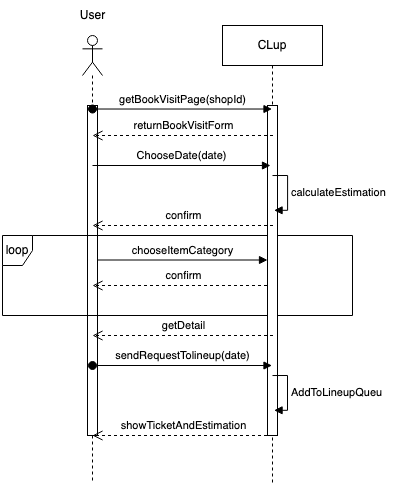
\includegraphics[width=0.7\textwidth,keepaspectratio]{images/BookAVisit_sd.png}
  \caption{Sequence diagram for book a visit}
\end{figure}

\begin{figure}[H]
  \centering
  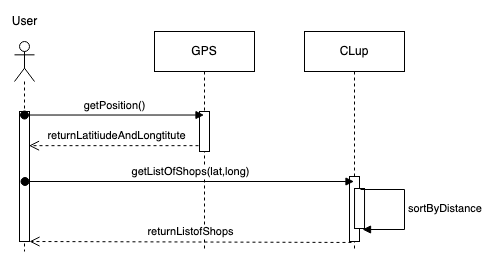
\includegraphics[width=0.8\textwidth,keepaspectratio]{images/SeeShopList_sd.png}
  \caption{Sequence diagram for see shop lists}
\end{figure}

\begin{figure}[H]
  \centering
  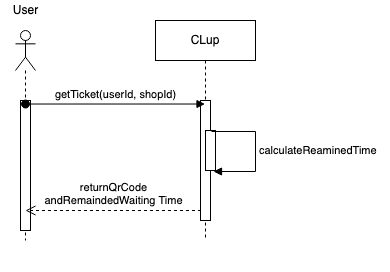
\includegraphics[width=0.6\textwidth,keepaspectratio]{images/GetTicket_sd.png}
  \caption{Sequence diagram for generate ticket}
\end{figure}

\begin{figure}[H]
  \centering
  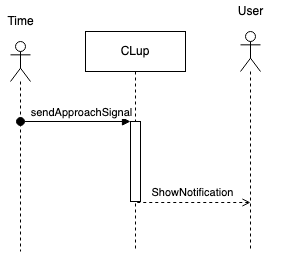
\includegraphics[width=0.5\textwidth,keepaspectratio]{images/NotifyApproach_sd.png}
  \caption{Sequence diagram for notify approach}
\end{figure}

\begin{figure}[H]
  \centering
  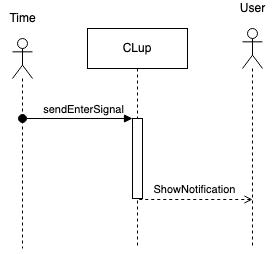
\includegraphics[width=0.5\textwidth,keepaspectratio]{images/NotifyCall_sd.png}
  \caption{Sequence diagram for notify call user turn}
\end{figure}

\begin{figure}[H]
  \centering
  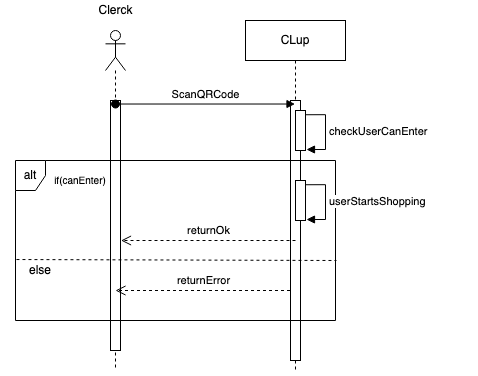
\includegraphics[width=0.7\textwidth,keepaspectratio]{images/ScanQREntrance_sd.png}
  \caption{Sequence diagram for scan for entrance}
\end{figure}

\begin{figure}[H]
  \centering
  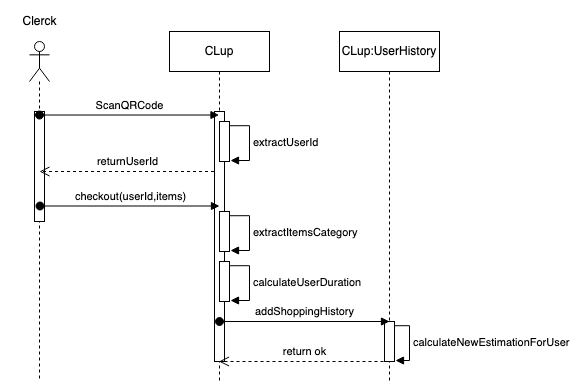
\includegraphics[width=0.9\textwidth,keepaspectratio]{images/Checkout_sd.png}
  \caption{Sequence diagram for user checkout}
\end{figure}

\begin{figure}[H]
  \centering
  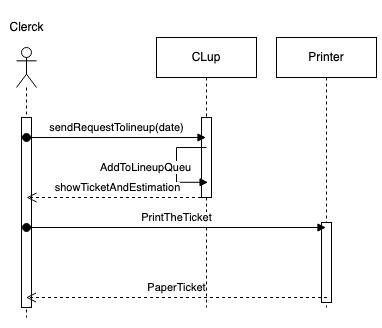
\includegraphics[width=0.7\textwidth,keepaspectratio]{images/PrintTicket_sd.png}
  \caption{Sequence diagram for clerk add offline user in queue}
\end{figure}
\clearpage

\setcounter{tocdepth}{3}
\setcounter{secnumdepth}{3}